\chapter{Технологическая часть}

В данном разделе производится выбор средств реализации, а также приводятся: описание подхода к сбору статистики, листинги реализованных алгоритмов, результаты тестирования программы.


\section{Выбор средств реализации}

Основное требование к языку программирования в данной лабораторной работе - наличие в нем нативных потоков. Язык C++ обладает этим свойством \cite{CBook} и уже использовался мною ранее, поэтому и был выбран. 

Для замеров времени используется предоставляемый класс system\_clock::time\_poin, использующий данные системных часов в реальном времени \cite{CBook2}, а для организации распараллеливания -  std::thread.

В качестве среды разработки выбран “QT Creator” так как он был часто использована мною ранее.

\section{Сбор статистки}

Чтобы наглядно показать, что ленты конвейра работают параллельно, в класс завок добавлены отметки времени поступления заявки в очередную очередь (или в пул обработанных задач) и времени покидания очередной очереди. В процессе обработки заявок конвейром в лог выводится информация о каждом подобном событии для каждой заявки.

На выходе, когда все заявки обработаны системой, собирается следующая статистика.
\begin{enumerate}[label={\arabic*)}]
	\item На сколько время обработки N заявок снижено в параллельной реализации конвейера по сравнению с последовательной обработкой одним потоком. Для этого перед запуском и после завершения каждой из реализаций запоминаются данные системных часов в реальном времени, затем второе время вычитается из первого, и получается время работы этой реализации. Далее показания реализаций сравниваются.
	
	\item Минимальное, максимальное и среднее время: проведенное заявкой в очереди, проведенное заявкой в системе. Для этого после обработки всех заявок для каждой из них вычисляется время, проведенной в каждой очереди, а также суммарные: время, проведенное в очередях и время, проведенное в системе. Затем вычисляется среднее, максимальное и минимальное каждого из этих значений среди всех заявок.
\end{enumerate}



\section{Реализация алгоритмов}

\lstset{language=C++}

В листинге \ref{meanl} представлены реализации рабочих потоков параллельного конвейера.

\begin{lstlisting}[caption=Реализация рабочих потоков параллельного конвейера,
	label={meanl}]
void Conveyor::find_mean(size_t n_tasks)
{
	size_t task_num = 0;
	
	while (task_num < n_tasks)
	{
		std::shared_ptr<Standardizer> task = q1.front();
		q1.pop();
		task->out1 = system_clock::now();
		
		task->find_mean(++task_num);
		
		m2.lock();
		q2.push(task);
		task->in2 = system_clock::now();
		m2.unlock();
	}
}
void Conveyor::find_std_dev(size_t n_tasks)
{
	size_t task_num = 0;
	
	while(task_num < n_tasks)
	{
		m2.lock();
		if (!this->q2.empty())
		{
			std::shared_ptr<Standardizer> task = q2.front();
			q2.pop();
			task->out2 = system_clock::now();
			m2.unlock();
			
			task->find_std_dev(++task_num);
			
			m3.lock();
			q3.push(task);
			task->in3 = system_clock::now();
			m3.unlock();
		}
		else
		m2.unlock();
	}
}
void Conveyor::transform(size_t n_tasks)
{
	size_t task_num = 0;
	
	while (task_num < n_tasks)
	{
		m3.lock();
		if (!this->q3.empty())
		{
			std::shared_ptr<Standardizer> task = q3.front();
			q3.pop();
			task->out3 = system_clock::now();
			m3.unlock();
			
			task->transform(++task_num);
			
			tasks.push_back(task);
			task->out_system = system_clock::now();
			
		}
		else
		m3.unlock();
	}
}
\end{lstlisting}

\newpage
В листинге \ref{main} представлена реализация главного потока параллельного конвейера.

\begin{lstlisting}[caption=Реализация главного потока параллельного конвейера,
	label={main}]
void Conveyor::run_parallel(size_t n_tasks, size_t n, double *arr, double *new_arr)
{
	for (size_t i = 0; i < n_tasks; i++)
	{
		std::shared_ptr<Standardizer> new_task(new Standardizer(n, arr, new_arr));
		q1.push(new_task);
		new_task->in1 = system_clock::now();
	}
	
	this->threads[0] = std::thread(&Conveyor::find_mean, this, n_tasks);
	this->threads[1] = std::thread(&Conveyor::find_std_dev, this, n_tasks);
	this->threads[2] = std::thread(&Conveyor::transform, this, n_tasks);
	
	for (size_t i = 0; i < numThreads; i++)
	{
		if (this->threads[i].joinable())
		this->threads[i].join();
	}
}
\end{lstlisting}

\newpage
В листинге \ref{linear} представлена реализация последовательной обработки данных одним потоком.

\begin{lstlisting}[caption=Реализация последовательной обработки данных одним потоком,
	label={linear}]
void Conveyor::run_linear(size_t n_tasks, size_t n, double *arr, double *new_arr)
{
	for (size_t i = 0; i < n_tasks; i++)
	{
		std::shared_ptr<Standardizer> task(new Standardizer(n, arr, new_arr));
		
		task->find_mean(i + 1);
		task->find_std_dev(i + 1);
		task->transform(i + 1);
		
		tasks.push_back(task);
	}
}
\end{lstlisting}

\newpage
\section{Тестирование}

Произведено тестирования алгоритма стандартизации программы по методу черного ящика: проведен запуск программного обеспечения для стандартизации массива из 10 элементов. Содержание массива до и после стандартизации приведено на рисунке  \ref{fig:work_example}. 

\begin{figure}[h!]
	
	\centering{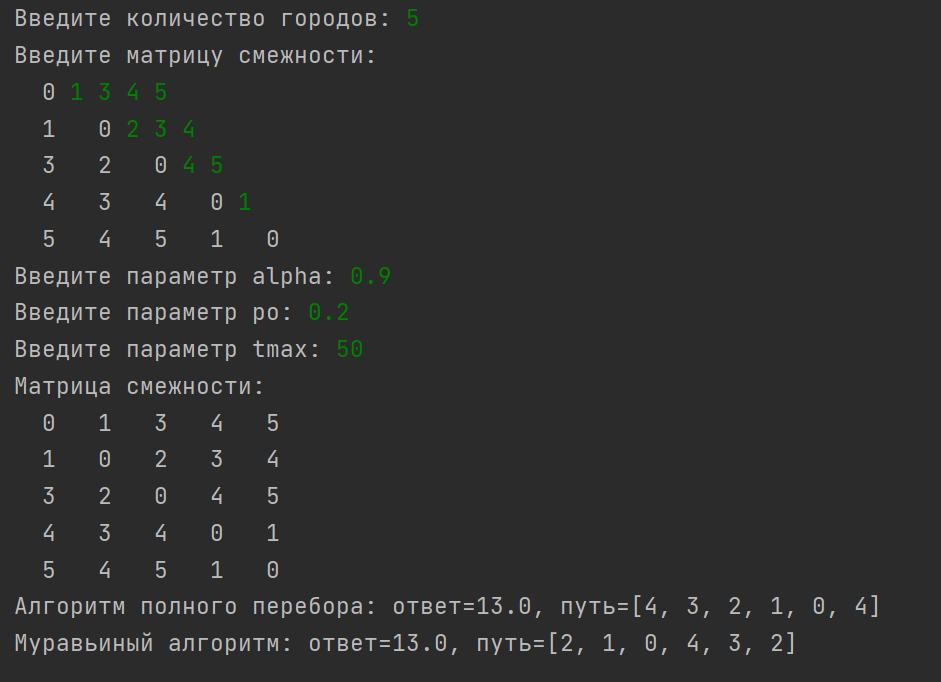
\includegraphics[scale=1]{inc/img/work_example.png}}
	
	\caption{Результат тестирования алгоритма стандартизации}
	
	\label{fig:work_example}
	
\end{figure}

Как видно на рисунке выше, цель стандартизации достигнута: получен массив с нулевым средним и стандартным отклонением, равным 1.

\newpage
На рисунке \ref{fig:work_example2} приведен пример вывода лога при обработке параллельным конвейером 5 заявок на стандартизацию массива из 100000 элементов.


\begin{figure}[h!]
	
	\centering{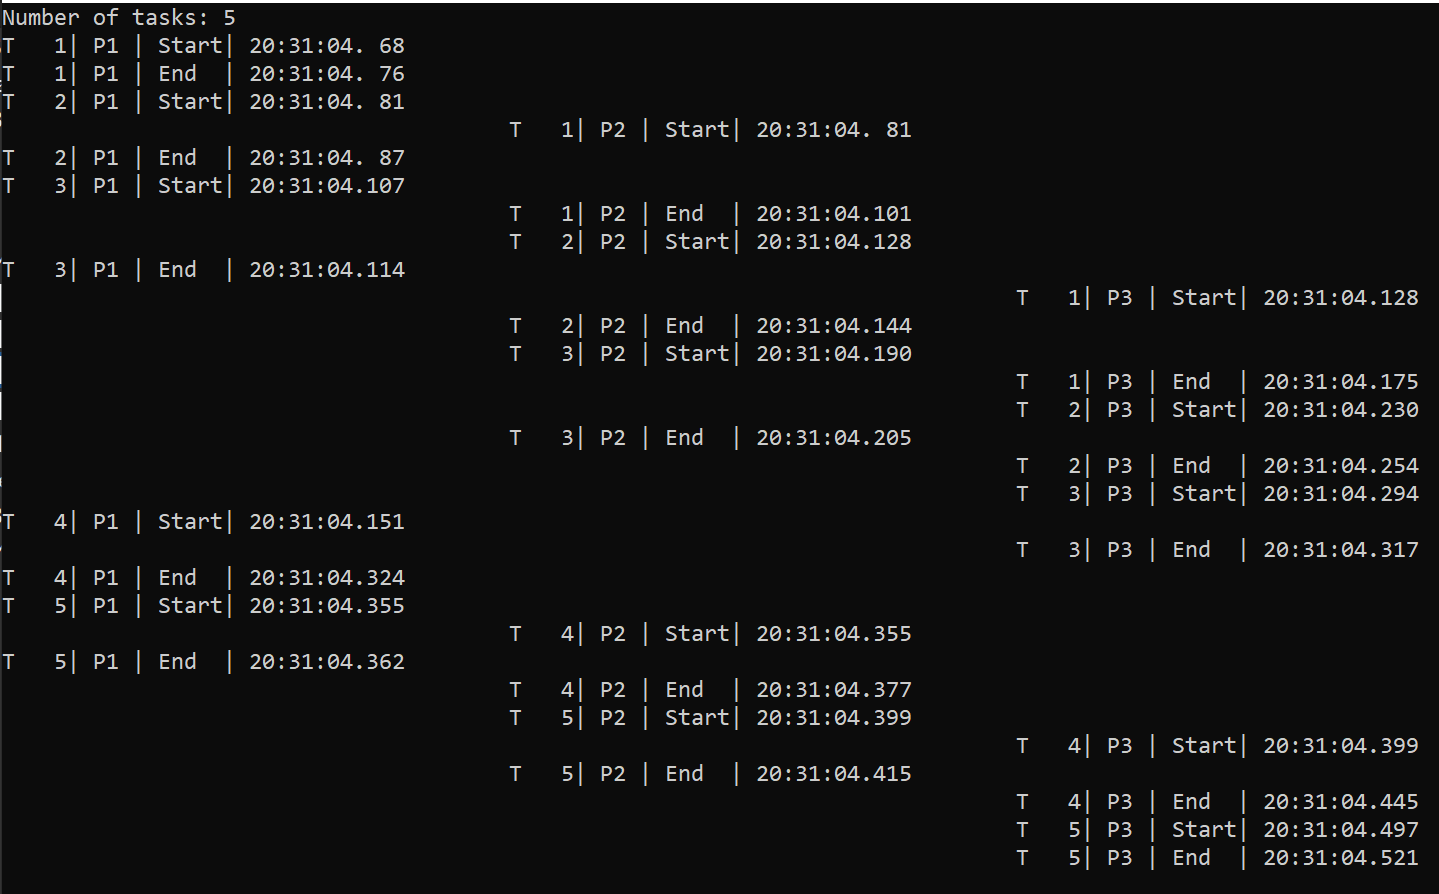
\includegraphics[scale=0.8]{inc/img/work_example2.png}}
	
	\caption{Результат логирования}
	
	\label{fig:work_example2}
	
\end{figure}


Как видно на рисунке выше, заявки действительно обрабатываются параллельно. Например, после завершения обработки первой заявки первым потоком, и ее помещения в очередь второго потока, параллельно начинается обработка второй заявки первым потоком и первой заявки вторым потоком.

На рисунке \ref{fig:stats2} приведен пример вывода собранной статистики при обработке параллельным конвейером 1000 заявок на стандартизацию массива из 100000 элементов.

\begin{figure}[h!]
	
	\centering{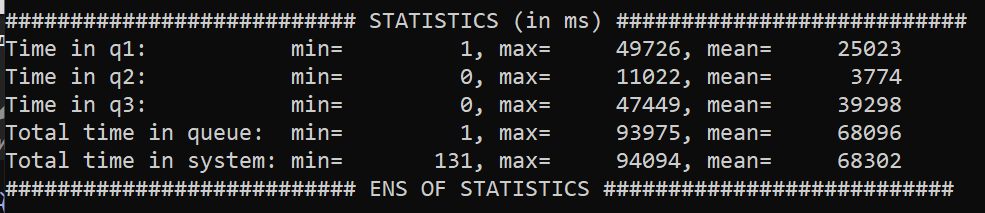
\includegraphics[scale=0.8]{inc/img/stats.png}}
	
	\caption{Пример собранной статистики}
	
	\label{fig:stats2}
	
\end{figure}


\newpage
На рисунке \ref{fig:work_example3} приведен пример вывода результатов сравнения времени выполнения при параллельной и линейной обработке 100 заявок на стандартизацию массива из 100000 элементов. 


\begin{figure}[h!]
	
	\centering{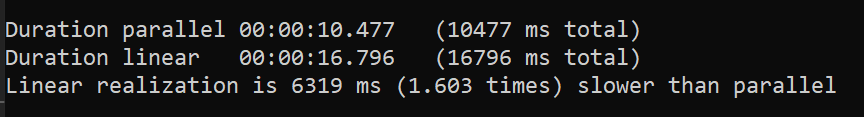
\includegraphics[scale=1]{inc/img/work_example3.png}}
	
	\caption{Результат сравнения времени выполнения параллельной и линейной реализаций}
	
	\label{fig:work_example3}
	
\end{figure}

Более подробно статистика и сравнение времени работы реализаций будут рассмотрены в следующем разделе.



\section{Вывод из технологической части}

Был произведен выбор средств реализации,  реализованы и протестированы последовательный и параллельный конвейерный подходы к стандартизации массива.
